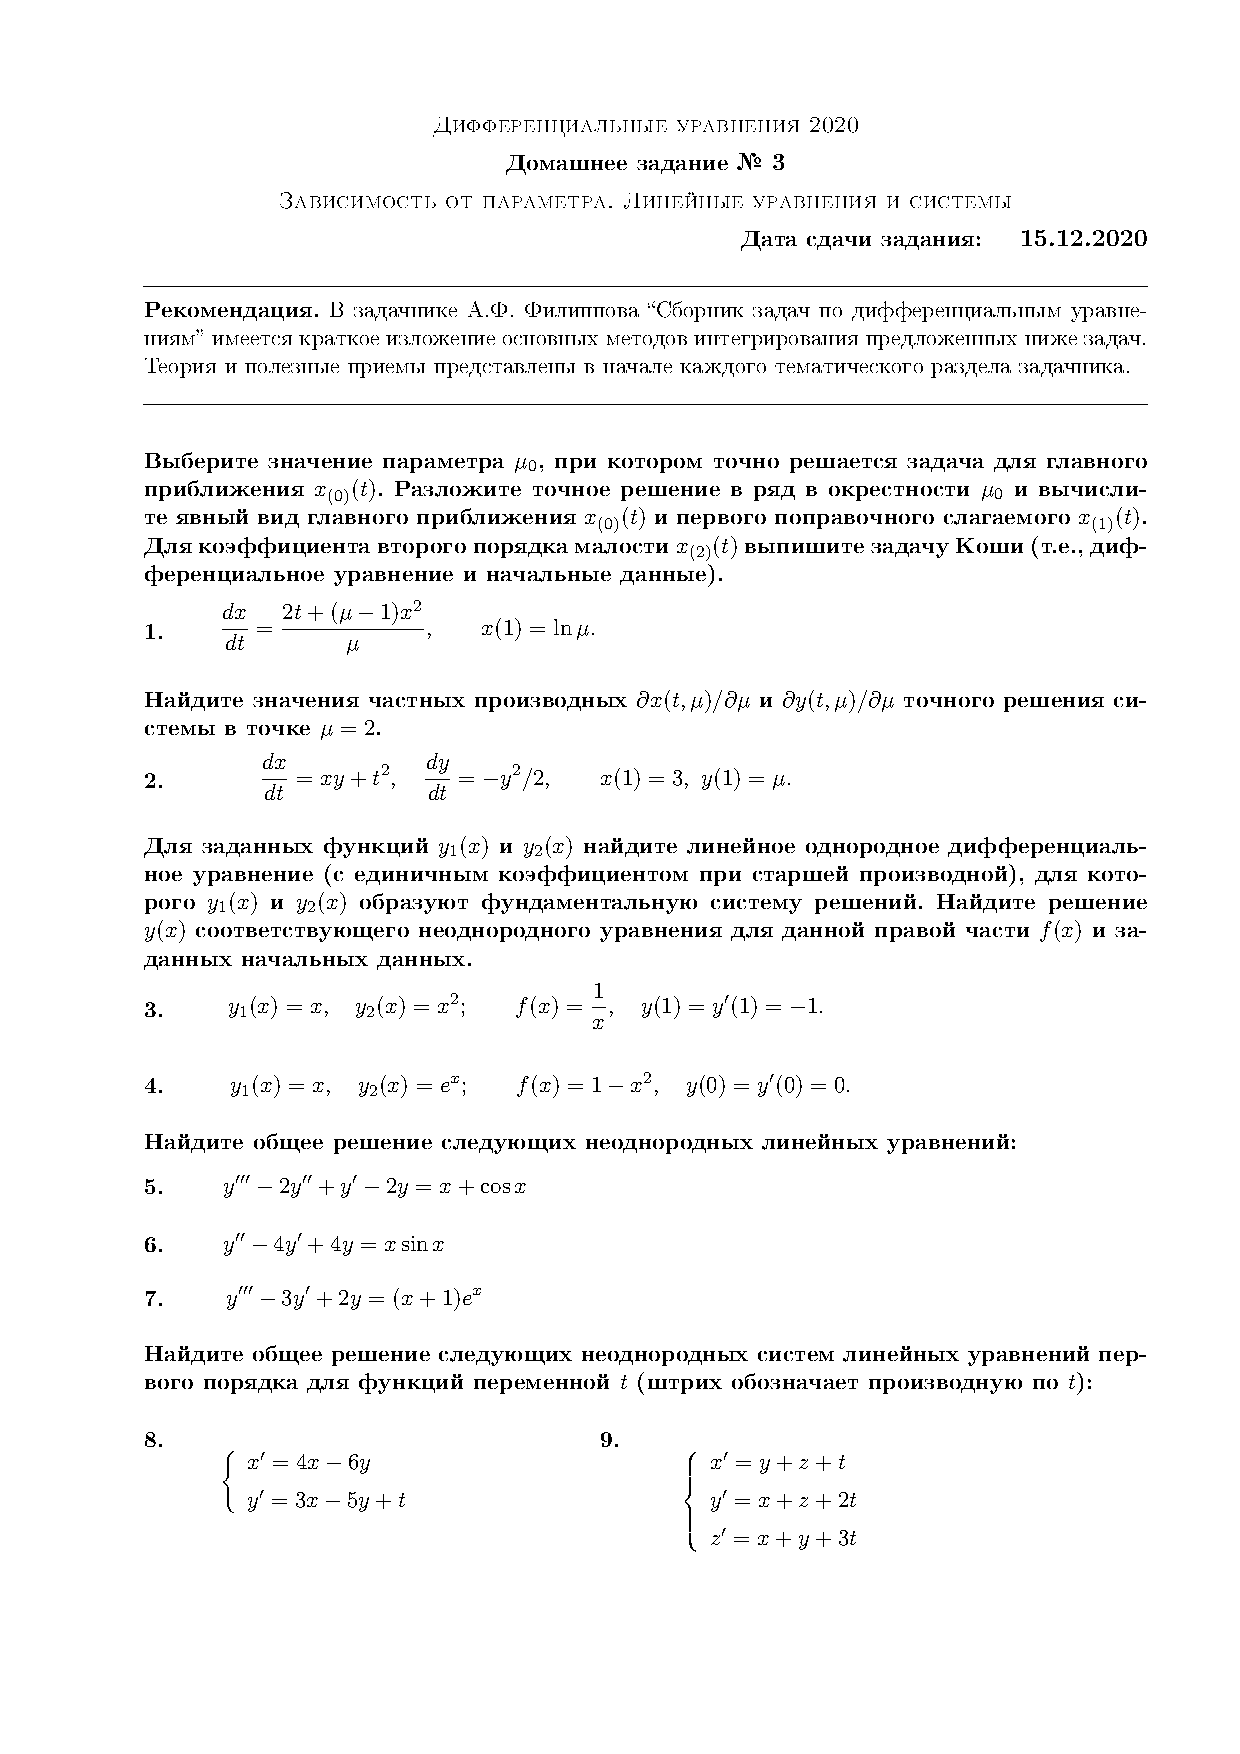
\includepdf[pages=1]{Tasks/HW-3-DE-2020}
\newpage
\section*{Решения}
\subsection*{Задача 1}
	\begin{gather*}
	\frac{d x}{d t} = \frac{2t + (\mu - 1)x^2}{\mu}\qquad x(1) = \ln(\mu)
	\end{gather*}
	Рассмотрим $\mu_0 = 1$
	\begin{gather*}
	\begin{cases}
	\dot{x} = 2t\ \Rightarrow\ x = t^2 + c\\
	x(1) = \ln(1) = 0
	\end{cases}\qquad x = t^2 - 1
	\end{gather*}
	Разложим в ряд вблизи $\mu = 1$
	\begin{gather*}
	x = x_0 + (\mu - 1)x_1 + \frac{(\mu - 1)^2}{2} x_2 + o(\mu^2)\\
	\dot{x} = \dot{x}_0 + (\mu - 1)\dot{x}_1 + \frac{(\mu - 1)^2}{2}\dot{x}_2 + o(\mu^2)\\
	x^2 = x^2_0 + (\mu - 1) 2x_0 x_1 + \frac{(\mu - 1)^2}{2}(2x_0x_2 + 2x_1^2) + o(\mu^2)\\
	\mu \dot{x} = 2t + (\mu - 1)x^2\qquad 1-\dot{x}\\
	(\mu - 1)\dot{x} = 2t + (\mu - 1)x^2 - \dot{x}
	\end{gather*}
	Рассмотрим $x(1)$
	\begin{gather*}
	x(1) = \ln(\mu) = \ln(1 + (\mu - 1)) = (\mu - 1) - \frac{(\mu - 1)^2}{2} + o(\mu^2)\\
	x_0(1) = 0\qquad x_1(1) = 1\qquad x_2(1) = -1
	\end{gather*}
	Составим задачи Коши
	\begin{enumerate}
	\item[$(\mu - 1)^0$] 
		\begin{gather*}
		\begin{cases}
		0 = 2t + 0 - \dot{x}_0\\
		x_0(1) = 0
		\end{cases}\\
		x_0 = t^2 - 1
		\end{gather*}
	\item[$(\mu - 1)^1$] 
		\begin{gather*}
		\begin{cases}
		\dot{x}_0 = x_0^2 - \dot{x}_1\\
		x_1(1) = 1
		\end{cases}\\
		\dot{x}_1 = (t^2 - 1)^2 - 2t = t^4 - 2t^2 - 2t + 1\\
		x_1 = \frac{t^5}{5} - \frac{2t^3}{3} - t^2 + t + c\\
		c = 1 - \frac{1}{5} + \frac{2}{3} + 1 - 1 = \frac{22}{15}
		\end{gather*}
	\item[$(\mu - 1)^2$]
		\begin{gather*}
		\begin{cases}
		\dot{x}_1 = 2x_0 x_1 - \dot{x}_2\\
		x_2(1) = -1
		\end{cases}\\
		\dot{x}_2 = 2(t^2-1)\left( \frac{t^5}{5} - \frac{2t^3}{3} - t^2 + t + \frac{22}{15} \right) - t^4 + 2t^2 + 2t - 1=\\
		\frac{2t^7}{5} - \frac{26t^5}{15} - 3t^4 + \frac{10t^3}{3} + \frac{104t^2}{15} - \frac{59}{15}
		\end{gather*}
	\end{enumerate}
	Тогда задача Коши для $x_2$
	\begin{gather*}
	\begin{cases}
	\dot{x}_2 = \frac{2t^7}{5} - \frac{26t^5}{15} - 3t^4 + \frac{10t^3}{3} + \frac{104t^2}{15} - \frac{59}{15}\\
	x_2(1) = -1
	\end{cases}
	\end{gather*}
\vskip 0.4in


\subsection*{Задача 2}
	\begin{gather*}
	\begin{cases}
		x(1) = 3\\
		y(1) = \mu = 2 + (\mu - 2)
	\end{cases}\\
	x(t,\mu) = x^{(0)}(t,2) + (\mu - 2)x^{(1)}(t) + \frac{(\mu - 2)^2}{2}x^{(2)}(t) + \ldots\\
	\mu^{(0)}:
	\begin{cases}
		\dot{y}^{(0)} = -\frac{y^{(0)^2}}{2}\qquad y^{(0)} = \frac{2}{t}\\
		\dot{x}^{(0)} = x^{(0)} y^{(0)} + t^2 = \frac{2x^{(0)}}{t} + t^2\qquad x^{(0)} = t^3 + 2t^2
	\end{cases}\\
	\frac{\partial y}{\partial t} = -\frac{y^2}{2}\qquad -\frac{1}{y} = -\frac{1}{2}t + \tilde{c}\qquad y = \frac{2}{t},\ y(1) = \mu = 2\\
	x' - \frac{2}{t} x = t^2\\
	x' - \frac{2}{t} x = 0\qquad \frac{\partial x}{\partial t} = \frac{2x}{t}\qquad \frac{1}{2}\ln(x) = \ln(t) + c\quad x = t^2 \tilde{c}\\
	\frac{\partial t^2 \tilde{c}(x)}{\partial t} = 2t \tilde{c}(x) + t^2 \tilde{c}'(x)\\
	2t\tilde{c}(x) + t^2\tilde{c}'(x) - 2t\tilde{c}(x) = t^2\qquad \tilde{c}'(x) = 1,\ \tilde{c}(x) = t + c\quad x = t^3 + 2t^2\\
	y^2 = (y^{(0)} + (\mu - 2)y^{(1)} + \frac{(\mu - 2)^2}{2!}y^{(2)}) = (y^{(0)})^2 + (\mu - 2)2y^{(0)}y^{(1)} + \frac{(\mu - 2)^2}{2}(2y^{(0)}y^{(2)} + (y^{(1)})^2) + \ldots\\
	\mu':
	\begin{cases}
		\dot{y}^{(1)} = -\frac{1}{2} 2 y^{(0)} y^{(1)} = -\frac{2}{t} y^{(1)}\qquad y^{(1)} = \frac{\tilde{c}}{t^2} = \frac{1}{t^2}\\
		\dot{x}^{(1)} = xy + t^2
	\end{cases}\\
	xy = (y^{(0)} + (\mu - 2)y^{(1)} + \ldots)(x^{(0)} + (\mu - 2)x^{(1)} + \ldots) =
	x^{(0)} y^{(0)} + (\mu - 2)(y^{(1)} x^{(0)} + y^{(0)} x^{(1)}) + \ldots\\
	\begin{cases}
		\dot{y}^{(1)} = \frac{2}{t^2}\\
		\dot{x}^{(1)} = t + 2 + x^{(1)} \frac{2}{t}
	\end{cases}\\
	\dot{x}^{(1)} - \frac{2}{t}x^{(1)} = t^2 + 2t\qquad x^{(1)} = \tilde{c}(t)t^2\\
	\frac{\partial \tilde{c}(t)t^2}{\partial t} = \tilde{c}'(t)t^2 + 2t\tilde{c}(t)\qquad
	\tilde{c}'(t)t^2 + 2t\tilde{c}(t) - 2t \tilde{c}(t) = t + 2\\
	\tilde{c}'(t) = \frac{1}{t} + \frac{2}{t^2}\qquad 
	\tilde{c}(t) = \ln(t) - \frac{2}{t} + c\\
	x^{(1)} = (\ln(t) - \frac{2}{t} + c)t^2\qquad
	x^{(1)}(1) = -2+c = 0\\
	x^{(1)} = (\ln(t) - \frac{2}{t} + 2)t^2
	\end{gather*}
\vskip 0.4in

\begin{comment}
	\begin{gather*}
x = x_0 + (\mu - 2)x_1 + \frac{(\mu - 2)^2}{2}x_2 + o(\mu^2)\qquad
\dot{x} = \dot{x}_0 + (\mu - 2)\dot{x}_1 + \frac{(\mu - 2)^2}{2}\dot{x}_2 + o(\mu^2)\\
y = y_0 + (\mu - 2)y_1 + \frac{(\mu - 2)}{2}y_2 + o(\mu^2)\qquad
\dot{y} = \dot{y}_0 + (\mu - 2)\dot{y}_1 + \frac{(\mu - 2)^2}{2}\dot{y}_2 + o(\mu^2)\\
xy - x_0y_0 + (\mu - 2)(x_0 y_1 + x_1 y_0) + \frac{(\mu - 2)^2}{2}(x_2 y_0 + 2x_1 y_1 + x_2 y_0) + o(\mu^2)\\
y^2 = y_0^2 + (\mu - 2)2y_0 y_1 + \frac{(\mu - 2)^2}{2} (2y_0 y_1 + 2y_1^2) + o(\mu^2)
\end{gather*}
Заметим что $\frac{(\mu - 2)^k}{k!}$ зануляется при дифференцировании по $\mu$ при $k = 2$\\
А значит $x'(2) = x_1,\ y'(2) = y_1$
\begin{enumerate}
\item[$(\mu - 2)^{0}$] 
\begin{gather*}
\begin{cases}
\dot{y}_0 = -\frac{y_0^2}{2}\\
y_0(1) = 2
\end{cases}
\qquad
\begin{cases}
\dot{x}_0 = x_0 y_0 + t^2\\
x_0(1) = 2
\end{cases}\\
\frac{d y_0}{d t} = \frac{y_0^2}{2}\\
-\frac{1}{y_0} = -\frac{t}{2} + c_1 = \frac{2c_1 - t}{2}
\qquad
y_0 = \frac{2}{t - c_0}
\qquad
y_0(1) = \frac{2}{1 - c_0} = 2
\qquad
\int \frac{d x_0}{x_0} = \int \frac{2dt}{t}\\
\ln|x_0| = 2\ln|t| + c_0\\
x_0 = ct^2
\qquad
x_0 = c(t) t^2\\
c'(t) \cdot t^2 + c(t) \cdot 2t = \frac{2}{t} \cdot c(t) \cdot t^2 + t^2
\qquad
c'(t) = 1
\qquad
c(t) = t + c_0\\
x_0 = t^2 (t + c_0) = t^3 + c_0 t^2 x_0(1) = 1 + c_0 = 3
\qquad
x_0 = t^3 + 2t^2
\end{gather*}
\item[$(\mu - 2)^{1}$]
\begin{gather*}
\begin{cases}
\dot{y}_1 = -\frac{2y_0 y_1}{2}\\
y_1(1) = 1
\end{cases}
\qquad
\begin{cases}
\dot{x}_1 = x_0 y_1 + x_1 y_0\\
x_1 (1) = 0
\end{cases}\\
\dot{y}_1 = - \frac{2}{t} y_1
\qquad
\int \frac{d y_1}{y_1} = -\int \frac{2dt}{t}\\
y_1 = \frac{c}{t^2}
\qquad
y_1(1) = c = 1
\qquad
y_1 = \frac{1}{t^2}\\
\dot{x}_1 = \frac{1}{t^2}(t^3 + 2t^2) + x_1 \cdot \frac{2}{t} = t + 2 + \frac{2x_1}{t}
\qquad
x_1 = c(t) t^2\\
c'(t) t^2 = t+2
\qquad
c'(t) = \frac{1}{t} + \frac{2}{t^2}
\qquad
c(t) = \ln(t) - \frac{2}{t} + c_0\\
x_1(1) = -2 + c_0 = 0
\qquad
x_1 = (\ln|t| - \frac{2}{t} + c_0) t^2
\qquad
x_1 = (\ln|t| - \frac{2}{t} + 2) t^2
\end{gather*}
\end{enumerate}
\end{comment}

\newpage
\subsection*{Задача 3}
	\begin{gather*}
		y_1(x) = x,\ y_2(x) = x^2\quad f(x) = \frac{1}{x}\quad y(1) = y'(1) = -1\\
		W_2[y_1,y_2] = 
		\begin{vmatrix}
			x & x^2\\
			1 & 2x
		\end{vmatrix}
		= x^2\\
		W_3[y_1,y_2,y_3] =
		\begin{vmatrix}
			x & x^2 & g\\
			1 & 2x & g'\\
			0 & 2 & g''
		\end{vmatrix}
		=
		2x^2 g'' + 2g  - 2xg' - x^2 g'' = 0\\
		x^2g'' - 2xg' + 2g = 0
	\end{gather*}
	Решим ДУ
	\begin{gather*}
	\begin{cases}
		y(x) = x^2 g'' - 2xg' + 2g - \frac{1}{x} = 0\\
		y(1) = y'(1) = -1
	\end{cases}\\
	\begin{pmatrix}
		x & x^2\\
		1 & 2x
	\end{pmatrix}
	\begin{pmatrix}
		c_1' \\ c_2'
	\end{pmatrix}
	=
	\begin{pmatrix}
		0 \\ \frac{1}{x}
	\end{pmatrix}\\
	y(x) = c_1(x)x + c_2(x)x^2\\
	\begin{pmatrix}
		xc_1' + x^2c_2' \\ c_1' + 2xc_2'
	\end{pmatrix}
	=
	\begin{pmatrix}
		0 \\ \frac{1}{x}
	\end{pmatrix}\\
	\begin{cases}
		xc_1' = -x^2c_2' \\ c_1' + 2xc_2'
	\end{cases}
	\qquad
	\begin{cases}
		c_1' = -xc_2' \\ \frac{1}{x}
	\end{cases}\\
	c_2' = \frac{1}{x^2}\qquad c_2 = -\frac{1}{x} + D_2\\
	c_1' = -\frac{1}{x}\qquad c_1 = -\ln(x) + D_1\\
	y(x) = (-\ln(x) + D_1)x + (-\frac{1}{x} + D_2)x^2 = -x\ln x + D_1 x - x + D_2 x^2\\
	y(1) = D_1 + D_2 - 1 = -1\quad D_1 + D_2 = 0\\
	y'(1) = -\ln(1) - 1 + D_1 + 2D_2 - 1 = -1\\
	\begin{cases}
		D_1 + D_2 = 0 \\ D_1 + 2D_2 = 1
	\end{cases}\qquad
	\begin{cases}
		D_1 = -1 \\ D_2 = 1
	\end{cases}\\
	y(x) = -x\ln x - 2x + x^2
	\end{gather*}
\vskip 0.4in


\subsection*{Задача 4}
	\begin{gather*}
	y_1(x) = x,\ y_2(x) = e^{x}\qquad
	f(x) = 1-x^2,\ y(0) = y'(0) = 0\\
	W_2[y_1,y_2] =
	\begin{vmatrix}
		x & e^x \\ 1 & e^x
	\end{vmatrix}
	=
	xe^x - e^x\\
	W_3[y_1,y_2,y] = 
	\begin{vmatrix}
		x & e^x & y\\
		1 & e^x & y'\\
		0 & e^x & y''
	\end{vmatrix}
	=
	xe^x y'' + e^x y - xe^x y' - e^x y'' =
	e^x\left((x-1)y'' - xy' + y\right) = 0
	\end{gather*}
	Решим ДУ
	\begin{gather*}
	\begin{cases}
		y(x) = e^x((x-1)y'' - xy' + y) = 1 - x^2\\
		y(0) = y'(0) = 0
	\end{cases}\\
	\begin{pmatrix}
		x & e^x \\ 1 & e^x
	\end{pmatrix}
	\begin{pmatrix}
		c_1' \\ c_2'
	\end{pmatrix}
	=
	\begin{pmatrix}
		0 \\ 1-x^2
	\end{pmatrix}\\
	y(x) = c_1(x)x + c_2(x)e^x\\
	\begin{cases}
		xc_1' + e^x c_2' = 0\\
		c_1' + e^xc_2' = 1-x^2
	\end{cases}\qquad
	\begin{cases}
		e^xc_2' = -xc_1'\\
		c_1'(1-x) = 1-x^2
	\end{cases}\\
	x = 1 \text{ или }\\
	c_1' = 1+x\qquad c_1 = x + \frac{1}{2}x^2 + D_1\\
	c_2' = (-x^2 - \frac{1}{2}x^3 - D_1x)e^{-x} =
	e^{-x}((x-2)x + \frac{1}{2}(x-3)x^2 + (x-1)D_1) + D_2\\
	y(x) = (x + \frac{1}{2}x^2 + D_1)x + (x-2)x + \frac{1}{2}(x-3)x^2 + (x-1)D_1 + D_2 e^x\\
	y(0) = D_2 = 0\\
	y'(0) = D_1 - 2 + D_1 + D_2 = 0\\
	y(x) = x^2 + \frac{1}{2}x^3 + x + x^2 - 2x + \frac{1}{2}x^3 - \frac{3}{2}x^2 + x - 1 = x^3 + \frac{1}{2}x^2 - 1
	\end{gather*}
\vskip 0.4in
	
	
\subsection*{Задача 5}
	\begin{gather*}
	y''' - 2y'' + y' - 2y = x + \cos x\\
	\lambda^3 - 2\lambda^2 + \lambda - 2 = 0\\
	(\lambda - 2)(\lambda^2 + 1) = 0\\
	\lambda_1 = 2,\ \lambda_2 = i,\ \lambda_3 = -i\\
	y(x) = c_1 e^{2x} + c_2 \sin(x) + c_3 \cos(x)\\
	\begin{pmatrix}
		e^{2x} & \sin(x) & \cos(x)\\
		2e^{2x} & \cos(x) & -\sin(x)\\
		4e^{2x} & -\sin(x) & -\cos(x)
	\end{pmatrix}
	\begin{pmatrix}
		c_1' \\ c_2' \\ c_3'
	\end{pmatrix}
	=
	\begin{pmatrix}
		0 \\ 0 \\ x + \cos(x)
	\end{pmatrix}\\
	\begin{cases}
		e^{2x}c_1' + \sin(x)c_2' + \cos(x)c_3' = 0\\
		2e^{2x}c_1' + \cos(x)c_2' - \sin(x)c_3' = 0\\
		4e^{2x}c_1' - \sin(x)c_2' - \cos(x)c_3' = x + \cos(x)
	\end{cases}\\
	(1) + (3) = 5e^{2x}c_1' = x + \cos(x)\qquad c_1'= \frac{1}{5}(x + \cos(x))e^{-2x}\\
	c_1 = -\frac{1}{100} e^{-2x} (10x-4\sin(x) + 8\cos(x) + 5) + A\\
	\begin{cases}
		\frac{1}{5}(x + \cos(x)) + \sin(x)c_2' + \cos(x)c_3' = 0\\
		\frac{2}{5}(x + \cos(x)) + \cos(x)c_2' - \sin(x)c_3' = 0
	\end{cases}\\	
	5c_2' = 2x \sin(x) - x \cos(x) + 2\sin(x)\cos(x) - \cos(x)^2\\
	c_2 = \frac{1}{10}(-x - 2(x-2)\sin(x) - 2 \cos(x)^2 - 4x\cos(x) - \sin(x)\cos(x) - 2\cos(x)) + B\\
	5c_3'= (2\cos(x) + \sin(x))(x + \cos(x))\\
	c_3 = -\frac{1}{10}(2x + 4x\sin(x) + 2\sin(x) - \cos(x)^2 - 2x\cos(x) + 2\sin(x)\cos(x) + 4\cos(x)) + C
	\end{gather*}
	Подставим в $y(x) = c_1 e^{2x} + c_2 \sin(x) + c_3 \cos(x)$
	\begin{gather*}
	y(x) = \left(-\frac{1}{100} e^{-2x} (10x-4\sin(x) + 8\cos(x) + 5) + A\right) e^{2x} +\\
	\left(\frac{1}{10}(-x - 2(x-2)\sin(x) - 2 \cos(x)^2 - 4x\cos(x) - \sin(x)\cos(x) - 2\cos(x)) + B\right) \sin(x) +\\
	\left(-\frac{1}{10}(2x + 4x\sin(x) + 2\sin(x) - \cos(x)^2 - 2x\cos(x) + 2\sin(x)\cos(x) + 4\cos(x)) + C\right) \cos(x) =
	\\ \\
	A e^{2x} + B \sin(x) + C \cos(x) - 
	\frac{1}{100} (10x-4\sin(x) + 8\cos(x) + 5) +\\
	\frac{1}{10} \sin(x) (-x - 2(x-2)\sin(x) - 2 \cos(x)^2 - 4x\cos(x) - \sin(x)\cos(x) - 2\cos(x)) -\\
	\frac{1}{10} \cos(x) (2x + 4x\sin(x) + 2\sin(x) - \cos(x)^2 - 2x\cos(x) + 2\sin(x)\cos(x) + 4\cos(x)) =
	\\ \\
	A e^{2x} + B \sin(x) + C \cos(x) - 
	\frac{10}{100}x + \frac{4}{100} \sin(x) - \frac{8}{100} \cos(x) - \frac{5}{100} -\\
	\frac{1}{10}x\sin(x) - \frac{2}{10}x\sin(x)^2 + \frac{4}{10}\sin(x)^2 - \frac{2}{10} \cos(x)^2\sin(x) - \frac{4}{10} x\cos(x)\sin(x) - \frac{1}{10}\sin(x)^2\cos(x) - \frac{2}{10}\cos(x) +\\
	\frac{2}{10} x\cos(x) - \frac{4}{10} x\sin(x)\cos(x) - \frac{2}{10} \sin(x)\cos(x) + \frac{1}{10}\cos(x)^3 + \frac{2}{10}x\cos(x)^2 - \frac{2}{10}\sin(x)\cos(x)^2 - \frac{4}{10}\cos(x)^2 =
	\\ \\
	A e^{2x} + B \sin(x) + C \cos(x) - \frac{1}{10}x + \frac{1}{25}\sin(x) - \frac{2}{25}\cos(x) - \frac{1}{20} - \frac{1}{10}x\cos(x) -\\
	\frac{2}{10}\cos(x)^3 - \frac{4}{10}x\cos(x)^2 - \frac{2}{10}\sin(x)^2 - \frac{2}{10}\sin(x)^2 \cos(x) =
	\end{gather*}
	\begin{gather*}
	A e^{2x} + B \sin(x) + C \cos(x) - \frac{2}{10} - \frac{4}{10}x - \frac{1}{10}x + \frac{1}{25}\sin(x) - \frac{2}{25}\cos(x)\\
	- \frac{1}{20} - \frac{1}{10}x\cos(x) - \frac{2}{10}x\sin(x) - \frac{2}{10}\sin(x)^2\cos(x) - \frac{2}{10}\cos(x)^3 =
	\\ \\
	A e^{2x} + B \sin(x) + C \cos(x) - \frac{1}{4} - \frac{1}{2}x + \frac{1}{25}\sin(x) - \frac{2}{25}\cos(x) - \frac{1}{10}x\cos(x) - \frac{2}{10}x\sin(x) - \frac{2}{10}\cos(x) =
	\\ \\
	A e^{2x} + B \sin(x) + C \cos(x) - \frac{1}{4} - \frac{1}{2}x - \frac{1}{10}x\cos(x) - \frac{2}{10}x\sin(x)
	\end{gather*}
	Ответ: 
	\begin{gather*}
	y(x) = 
	A e^{2x} + B \sin(x) + C \cos(x) - \frac{1}{4} - \frac{1}{2}x - \frac{1}{10}x\cos(x) - \frac{2}{10}x\sin(x)
	\end{gather*}
\vskip 0.4in


\subsection*{Задача 6}
	\begin{gather*}
	y'' - 4y'+ 4y = x \sin x\\
	\lambda^2 - 4\lambda + 4 = 0\\
	(\lambda - 2)^2 = 0\\
	\lambda_{1,2} = 2\\
	y(x) = c_1 e^{2x} + c_2 xe^{2x}\\
	\begin{pmatrix}
		e^{2x} & xe^{2x}\\
		2e^{2x} & (2x+1)e^{2x}
	\end{pmatrix}
	\begin{pmatrix}
		c_1' \\ c_2'
	\end{pmatrix}
	=
	\begin{pmatrix}
		0 \\ x\sin(x)
	\end{pmatrix}\\
	\begin{cases}
		e^{2x}c_1' + xe^{2x}c_2' = 0\\
		2e^{2x}c_1' + (2x+1)e^{2x}c_2' = x \sin(x)
	\end{cases}\\
	(2) - 2(1) = e^{2x}c_2' = x\sin(x)\qquad c_2' = x\sin(x) e^{-2x}\\
	(1):\ e^{2x}c_1' + x^2 \sin(x) = 0\qquad c_1'= -x^{2}\sin(x) e^{-2x}\\
	c_2 = -\frac{1}{25}e^{-2x} \left(\left(10x + 3\right)\sin(x) + \left(5x + 4\right)\cos(x)\right) + B\\
	c_1 = \frac{1}{125}e^{-2x} \left((50x^2 + 30x + 4)\sin(x) + (25x^2 + 40x + 22)\cos(x)\right) + A
	\end{gather*}
	Подставим в $y(x) = c_1 e^{2x} + c_2 xe^{2x}$
	\begin{gather*}
	y(x) = \left(\frac{1}{125}e^{-2x} \left((50x^2 + 30x + 4)\sin(x) + (25x^2 + 40x + 22)\cos(x)\right) + A\right)\cdot e^{2x} + \\
	\left(-\frac{1}{25}e^{-2x} \left(\left(10x + 3\right)\sin(x) + \left(5x + 4\right)\cos(x)\right) + B\right) \cdot x e^{2x} =
	\\
	A e^{2x} + B x e^{2x} + \frac{1}{125} \left((50x^2 + 30x + 4)\sin(x) + (25x^2 + 40x + 22)\cos(x)\right) -
	\frac{1}{25} x \left(\left(10x + 3\right)\sin(x) + \left(5x + 4\right)\cos(x)\right) =
	\\
	A e^{2x} + B x e^{2x} + \sin(x) \left(\frac{50x^2 + 30x + 4}{125} - \frac{10x^2 + 3x}{25}\right) + \cos(x) \left(\frac{25x^2 + 40x + 22}{125} - \frac{5x^2 + 4x}{25}\right) =
	\\
	A e^{2x} + B x e^{2x} + \sin(x) \frac{15x + 4}{125} + \cos(x) \frac{20x + 22}{125}
	\\
	y(x) = A e^{2x} + B x e^{2x} + \frac{3}{25}x \sin(x) + \frac{4}{125} \sin(x) + \frac{4}{25} x \cos(x) + \frac{22}{125}\cos(x)
	\end{gather*}
\vskip 0.4in


\subsection*{Задача 7}
	\begin{gather*}
	y''' - 3y' + 2y = (x+1)e^x\\
	\lambda^3 - 3\lambda + 2 = 0\\
	(\lambda - 1)^2(\lambda + 2) = 0\\
	\lambda_1 = 1,\ \lambda_2 = 1,\ \lambda_3 = -2\\
	y(x) = c_1 e^{x} + c_2 xe^{x} + c_3 e^{-2x}\\
	\begin{pmatrix}
		e^{x} & xe^{x} & e^{-2x}\\
		e^{x} & (x+1)e^{x} & -2e^{-2x}\\
		e^{x} & (x+2)e^{x} & 4e^{-2x}
	\end{pmatrix}
	\begin{pmatrix}
		c_1' \\ c_2' \\ c_3'
	\end{pmatrix}
	=
	\begin{pmatrix}
		0 \\ 0 \\ (x+1)e^{x}
	\end{pmatrix}\\
	\begin{cases}
		e^{x}c_1' + xe^{x}c_2' + e^{-2x}c_3' = 0\\
		e^{x}c_1' + (x+1)e^{x}c_2' - 2e^{-2x}c_3' = 0\\
		e^{x}c_1' + (x+2)e^{x}c_2' + 4e^{-2x}c_3' = (x + 1)e^{x}
	\end{cases}\\
	(3) + (1) - 2(2) = 9 e^{-2x}c_3' = (x+1)e^x\qquad c_3'= \frac{1}{9}(x+1)e^{3x}\\
	c_3 = \frac{1}{81}(3x+2)e^{3x}\\
	(3) - (2) = e^{x}c_2' + \frac{2+4}{9}e^x (x+1) = (x+1)e^x\qquad c_2' = \frac{1}{3}(x+1)\\
	c_2 = \frac{1}{3} \left(\frac{x^2}{2} + x\right)\\
	(2) = e^x c_1' + (x+1)e^x \cdot \frac{1}{3}(x+1) - 2e^{-2x} \cdot \frac{1}{9}(x+1)e^{3x} =\\
	e^x c_1' + \frac{1}{3}e^{x}(x+1)^2 - \frac{2}{9}e^x (x+1) =\\
	e^x c_1' + \frac{1}{9} e^x (3x^2 + 4x + 1)\qquad c_1' = -\frac{1}{9}(3x^2 + 4x + 1)\\
	c_1 = -\frac{1}{9}x(x+1)^2
	\end{gather*}
	Подставим в $y(x) = c_1 e^{x} + c_2 xe^{x} + c_3 e^{-2x}$
	\begin{gather*}
	y(x) = \left(-\frac{1}{9}x(x+1)^2 + A\right) \cdot e^x + \left(\frac{1}{3} \left(\frac{x^2}{2} + x\right) + B\right) \cdot xe^x + \left( \frac{1}{81}(3x+2)e^{3x} + C\right) \cdot e^{-2x} =
	\\
	A e^{x} + B x e^{x} + C e^{-2x} - \frac{1}{9} x(x+1)^2 e^x + \frac{1}{3} xe^x \left(\frac{x^2}{2} + x\right) + \frac{1}{81}(3x+2)e^x =
	\\
	A e^{x} + B x e^{x} + C e^{-2x} - \frac{1}{9}e^x (x^3 + 2x^2 + x) + e^x(\frac{1}{6}x^3 + \frac{1}{3}x^2) + \frac{1}{81}e^x(3x+2)\\
	y(x) = A e^{x} + B x e^{x} + C e^{-2x} + \frac{1}{18}x^3 e^x + \frac{1}{9} x^2 e^x
	\end{gather*}
\vskip 0.4in


\subsection*{Задача 8}
	\begin{gather*}
	\begin{cases}
	x' = 4x - 6y\\
	y' = 3x - 5y + t
	\end{cases}\\
	\dot{X} = AX + F(t)\\
	A = 
	\begin{pmatrix}
		4 & -6\\
		3 & -5
	\end{pmatrix}
	\qquad
	F = 
	\begin{pmatrix}
		0 \\ t
	\end{pmatrix}\\
	\begin{vmatrix}
		4-\lambda & -6\\
		3 & -5-\lambda
	\end{vmatrix}
	= (\lambda - 1)(\lambda + 2)\qquad \det(E - A) = 0\quad \det(-2E - A) = 0\\
	A - E = 
	\begin{pmatrix}
		3 & -6\\
		3 & -6
	\end{pmatrix}
	u_0 = 0\qquad
	u_0 = 
	\begin{pmatrix}
		2 \\ 1
	\end{pmatrix}\\
	A + 2E = 
	\begin{pmatrix}
		6 & -6\\
		3 & -3
	\end{pmatrix}
	u_1 = 0\qquad
	u_1 = 
	\begin{pmatrix}
		1 \\ 1
	\end{pmatrix}\\
	X_{\text{ч}}(t) = 
	\begin{pmatrix}
		\alpha_0 t + \alpha_1\\
		\beta_0 t + \beta_1
	\end{pmatrix}\\
	\begin{pmatrix}
		\alpha_0 \\ \beta_0
	\end{pmatrix}
	= \dot{X} = AX + F =
	\begin{pmatrix}
		t(4\alpha_0 - 6\beta_0) + (4\alpha_1 - 6\beta_1)\\
		t(3\alpha_0 - 5\beta_0 + 1) + (3\alpha_1 - 5\beta_1)
	\end{pmatrix}\\
	\alpha_0 = 3,\ \beta_0 = 2,\ \alpha_1 = \frac{3}{2},\ \beta_1 = \frac{1}{2}\\
	X(t) = 
	\begin{pmatrix}
		3t + \frac{3}{2}\\
		2t + \frac{1}{2}
	\end{pmatrix}
	+
	A e^{t}
	\begin{pmatrix}
		2 \\ 1
	\end{pmatrix}
	+
	B e^{-2t}
	\begin{pmatrix}
		1 \\ 1
	\end{pmatrix}
	\end{gather*}
\vskip 0.4in


\subsection*{Задача 9}
	\begin{gather*}
	\begin{cases}
	x' = y + z + t\\
	y' = x + z + 2t\\
	z'= x + y + 3t
	\end{cases}\\
	\dot{X} = AX + F(t)\\
	A = 
	\begin{pmatrix}
		0 & 1 & 1\\
		1 & 0 & 1\\
		1 & 1 & 0
	\end{pmatrix}
	\qquad
	F = 
	\begin{pmatrix}
		t \\ 2t \\ 3t
	\end{pmatrix}\\
	\begin{vmatrix}
		-\lambda & 1 & 1\\
		1 & -\lambda & 1\\
		1 & 1 & -\lambda
	\end{vmatrix}
	=
	-\lambda^3 + 2 + 3 \lambda = -(\lambda - 2)(\lambda + 1)^2\qquad \det(-E - A) = 0\quad \det(2E - A) = 0\\
	A + E = 
	\begin{pmatrix}
		1 & 1 & 1\\
		1 & 1 & 1\\
		1 & 1 & 1
	\end{pmatrix}
	u = 0\qquad
	u = 
	\begin{pmatrix}
		-x_2-x_3 \\ x_2 \\ x_3
	\end{pmatrix}\\
	u_0 
	\begin{pmatrix}
		-1 \\ 1 \\ 0
	\end{pmatrix}
	+ u_1
	\begin{pmatrix}
		-1 \\ 0 \\ 1
	\end{pmatrix}\\
	A - 2E = 
	\begin{pmatrix}
		-2 & 1 & 1\\
		1 & -2 & 1\\
		1 & 1 & -2
	\end{pmatrix}
	u_2 = 0\qquad
	u_2 = 
	\begin{pmatrix}
		1 \\ 1 \\ 1
	\end{pmatrix}\\
	X_{\text{ч}}(t) = 
	\begin{pmatrix}
		\alpha_0 t + \alpha_1\\
		\beta_0 t + \beta_1\\
		\gamma_0 t + \gamma_1
	\end{pmatrix}\\
	\begin{pmatrix}
		\alpha_0 \\ \beta_0 \\ \gamma_0
	\end{pmatrix}
	= \dot{X} = AX + F =
	\begin{pmatrix}
		t(\beta_0 + \gamma_0 + 1) + (\beta_1 + \gamma_1)\\
		t(\alpha_0 + \gamma_0 + 2) + (\alpha_1 + \gamma_1)\\
		t(\alpha_0 + \beta_0 + 3) + (\alpha_1 + \beta_1)
	\end{pmatrix}\\
	\alpha_0 = -2,\ \beta_0 = -1,\ \gamma_0 = 0,\ \alpha_1 = \frac{1}{2},\ \beta_1 = -\frac{1}{2},\ \gamma_1 = -\frac{3}{2}\\
	X(t) = 
	\begin{pmatrix}
		-2t + \frac{1}{2} \\ -t - \frac{1}{2} \\ -\frac{3}{2}
	\end{pmatrix}
	+ A e^{-t}
	\begin{pmatrix}
		-1 \\ 1 \\ 0
	\end{pmatrix}
	+ B e^{-t}
	\begin{pmatrix}
		-1 \\ 0 \\ 1
	\end{pmatrix}
	+ C e^{2t}
	\begin{pmatrix}
		1 \\ 1 \\ 1
	\end{pmatrix}
	\end{gather*}